\documentclass[aspectratio=169,11pt]{beamer}

\usepackage[utf8]{inputenc}
\usepackage[T1]{fontenc}
\usepackage[italian]{babel}
\usepackage{amsmath}
\usepackage{booktabs}
\usepackage{array}
\usepackage{tabularx}
\usepackage{graphicx}
\usepackage{ragged2e}
\usepackage{tikz}
\usetikzlibrary{arrows}

\usetheme{Madrid}
\usecolortheme{dove}
\setbeamertemplate{navigation symbols}{}
\setbeamertemplate{footline}[frame number]

\definecolor{UniudBlue}{RGB}{17,52,86}
\definecolor{UniudAccent}{RGB}{145,42,42}
\setbeamercolor{normal text}{fg=black,bg=white}
\setbeamercolor{structure}{fg=UniudBlue}
\setbeamercolor{title}{fg=black}
\setbeamercolor{titlelike}{fg=black,bg=white}
\setbeamercolor{frametitle}{fg=black,bg=black!4}
\setbeamercolor{palette primary}{fg=black,bg=black!6}
\setbeamercolor{palette secondary}{fg=black,bg=black!6}
\setbeamercolor{palette tertiary}{fg=black,bg=black!6}
\setbeamercolor{palette quaternary}{fg=black,bg=black!6}
\setbeamercolor{author in head/foot}{fg=black,bg=black!6}
\setbeamercolor{title in head/foot}{fg=black,bg=black!6}
\setbeamercolor{date in head/foot}{fg=black,bg=black!6}
\setbeamercolor{block title}{fg=white,bg=UniudBlue}
\setbeamercolor{block body}{fg=black,bg=UniudBlue!6}
\setbeamercolor{block title alerted}{fg=white,bg=UniudAccent}
\setbeamercolor{block body alerted}{fg=black,bg=UniudAccent!8}
\setbeamercolor{alerted text}{fg=UniudAccent}

\graphicspath{{figures/}{figures/results/}{resources/}}

\newcommand{\Fzero}{F_0}
\newcommand{\codepath}[1]{\texttt{#1}}

\title[Cardinalit\`a distinta nei data stream distribuiti]{Stima della cardinalit\`a distinta nei data stream distribuiti\\\large Algoritmi di sketching, framework sperimentale e merge semanticamente corretto}
\subtitle{Seminario magistrale}
\author{Daniele Ferroli}
\institute{Universit\`a degli Studi di Udine}
\date{A.A. 2024--2025}

\begin{document}

\begin{frame}
  \titlepage
\end{frame}

\begin{frame}{Roadmap del seminario}
  \begin{enumerate}
    \item Problema, modello minimo e vincoli del count-distinct
    \item Stato dell'arte: da Probabilistic Counting a HyperLogLog++
    \item Implementazione: architettura, hash, dataset e validazione
    \item Disegno sperimentale in modalit\`a streaming e merge
    \item Risultati principali su accuratezza, robustezza e compatibilit\`a semantica
    \item Conclusioni, limiti e sviluppi futuri
  \end{enumerate}
\end{frame}

\begin{frame}{Problema e contributo del lavoro}
  \begin{itemize}
    \item Obiettivo: stimare quanti identificatori distinti compaiono in un flusso continuo senza conservare tutto l'input.
    \item Applicazioni tipiche: monitoraggio di rete, telemetria, osservabilit\`a, analisi di log, ottimizzazione di interrogazioni.
    \item Nei sistemi distribuiti non basta stimare bene in locale: serve anche combinare sketch prodotti su nodi o partizioni diverse.
    \item La tesi non propone un nuovo stimatore teorico, ma uno studio sistematico del comportamento reale degli sketch e del loro merge.
  \end{itemize}

  \begin{block}{Contributo principale}
    Implementazione uniforme di pi\`u algoritmi count-distinct, interfaccia comune per le hash, framework riproducibile e distinzione esplicita tra casi \texttt{valid}, \texttt{recoverable} e \texttt{invalid}.
  \end{block}
\end{frame}

\begin{frame}{Modello minimo: stream, \(\Fzero\) e sketch}
  \begin{columns}[T,totalwidth=\textwidth]
    \column{0.56\textwidth}
      \begin{itemize}
        \item Il flusso \`e una sequenza ordinata \(S=\langle x_1,x_2,\dots,x_s\rangle\).
        \item Il lavoro assume il modello \emph{insertion-only}: ogni aggiornamento aggiunge occorrenze, non le rimuove.
        \item Gli algoritmi devono lavorare in uno o pochi passaggi, con memoria sublineare e aggiornamenti rapidi.
        \item Nel framework esiste anche un riferimento esatto interno, \codepath{NaiveCounting}, usato per test e controlli.
      \end{itemize}
    \column{0.44\textwidth}
      \[
        \Fzero = \left|\left\{a \in \mathcal{U} \mid f(a) > 0\right\}\right|
      \]
      \vspace{0.2cm}
      \begin{block}{Interpretazione}
        \(\Fzero\) \`e la cardinalit\`a del supporto del vettore delle frequenze, cio\`e il numero di elementi distinti osservati.
      \end{block}
      \begin{alertblock}{Vincolo di fondo}
        Il conteggio esatto non scala bene quando il flusso cresce; da qui nasce l'uso di sketch probabilistici.
      \end{alertblock}
  \end{columns}
\end{frame}

\begin{frame}{Evoluzione storica dello stato dell'arte}
  \small
  \begin{tabularx}{\textwidth}{>{\RaggedRight\arraybackslash}p{2.6cm} >{\RaggedRight\arraybackslash}X >{\RaggedRight\arraybackslash}p{3.8cm}}
    \toprule
    Metodo & Idea dominante & Ruolo nella tesi \\
    \midrule
    Probabilistic Counting & Bitmap singola che osserva eventi rari sull'hash & Primo punto della linea storica e benchmark implementato \\
    PCSA & Mediazione stocastica su pi\`u bitmap virtuali & Passo intermedio ricostruito nello stato dell'arte \\
    LogLog & Registri e media geometrica dei massimi di rango & Benchmark implementato \\
    HyperLogLog & Media armonica e correzioni di regime & Benchmark implementato e riferimento vicino a HLL++ \\
    HyperLogLog++ & Bias correction + stato sparso/denso & Riferimento pratico principale per gli esperimenti di merge \\
    \bottomrule
  \end{tabularx}

  \vspace{0.2cm}
  \small Lo stato dell'arte richiama anche Bloom filter e Count-Min Sketch per mostrare che lo sketching si estende oltre il solo conteggio dei distinti.
\end{frame}

\begin{frame}{Algoritmi implementati nel framework}
  \begin{columns}[T,totalwidth=\textwidth]
    \column{0.53\textwidth}
      \scriptsize
      \begin{tabular}{lll}
        \toprule
        ID & Metodo & Ruolo \\
        \midrule
        \texttt{naive} & NaiveCounting & riferimento esatto interno \\
        \texttt{pc} & Probabilistic Counting & benchmark pubblico \\
        \texttt{ll} & LogLog & benchmark pubblico \\
        \texttt{hll} & HyperLogLog & benchmark pubblico \\
        \texttt{hllpp} & HyperLogLog++ & benchmark pubblico \\
        \bottomrule
      \end{tabular}
    \column{0.47\textwidth}
      \scriptsize
      \begin{itemize}
        \item Interfaccia comune con \texttt{process}, \texttt{count}, \texttt{merge} e \texttt{reset}.
        \item La funzione di hash \`e iniettata nel costruttore e fa parte del contesto dello sketch.
        \item HLL++ \`e l'implementazione pi\`u articolata: stato sparso/denso, tabelle di bias, riduzione esplicita alla precisione minima.
      \end{itemize}
  \end{columns}
\end{frame}

\begin{frame}{Sketch, hash e mergeabilit\`a}
  \begin{itemize}
    \item Uno \emph{sketch} mantiene una sintesi compatta del flusso e permette di stimare \(\Fzero\) senza conservare tutti gli elementi.
    \item Negli sketch count-distinct l'hash non serve solo a randomizzare: determina come il flusso viene codificato nello stato.
    \item Uno sketch \`e \emph{mergeabile} se combinare due stati equivale a elaborare serialmente l'unione dei due flussi, a parit\`a di semantica o con degradazione esplicita.
  \end{itemize}

  \[
    \hat{\theta}\bigl(\mathcal{K}(S_1)\oplus\mathcal{K}(S_2)\bigr)
    \approx
    \hat{\theta}\bigl(\mathcal{K}(S_1 \cdot S_2)\bigr)
  \]

  \[
    \bigl(\mathcal{K}(S_1)\oplus\mathcal{K}(S_2)\bigr)[j]
    =
    \max\{\mathcal{K}(S_1)[j],\mathcal{K}(S_2)[j]\}
  \]

  \begin{alertblock}{Punto critico}
    Per gli sketch HLL-like il merge a massimi \`e corretto solo se i due lati condividono parametri compatibili e la stessa semantica dell'hash.
  \end{alertblock}
\end{frame}

\begin{frame}{Compatibilit\`a semantica del merge}
  \begin{columns}[T,totalwidth=\textwidth]
    \column{0.33\textwidth}
      \begin{block}{\texttt{valid}}
        Il merge \`e corretto direttamente.

        Caso tipico: HLL++ con stessa precisione, stessa funzione di hash e stesso seed.
      \end{block}
    \column{0.33\textwidth}
      \begin{block}{\texttt{recoverable}}
        Il merge non \`e corretto subito, ma lo diventa dopo una normalizzazione esplicita.

        Caso tipico: HLL++ con precisioni diverse ma stessa semantica dell'hash.
      \end{block}
    \column{0.33\textwidth}
      \begin{block}{\texttt{invalid}}
        In questo quadro non esiste un merge semanticamente corretto.

        Caso tipico: funzioni di hash o seed diversi.
      \end{block}
  \end{columns}

  \vspace{0.15cm}
  \small
  \begin{itemize}
    \item Strategia operativa distinta dalla compatibilit\`a: \texttt{direct}, \texttt{reject}, \texttt{reduce\_then\_merge}.
    \item \texttt{unsafe\_naive\_merge} viene mantenuto solo come controllo negativo sperimentale.
  \end{itemize}
\end{frame}

\begin{frame}{Architettura generale del sistema}
  \centering
  \resizebox{0.88\textwidth}{!}{\begin{tikzpicture}[x=1cm,y=1cm,>=latex,font=\small]
    \tikzstyle{module}=[draw, rounded corners=3pt, thick, align=center,
        text width=3.6cm, minimum height=1.35cm, inner sep=5pt]
    \tikzstyle{artifact}=[draw, rounded corners=3pt, thick, align=center,
        text width=3.8cm, minimum height=1.35cm, inner sep=5pt]
    \tikzstyle{flow}=[->, thick]
    \tikzstyle{support}=[->, thick, gray!80]

    % Layer frames
    \draw[dashed, rounded corners=6pt, gray!70] (-2.1,7.3) rectangle (23.9,10.2);
    \node[anchor=west, gray!70] at (-1.9,10.0) {\textbf{Tooling esterno}};

    \draw[dashed, rounded corners=6pt, gray!70] (-2.1,3.4) rectangle (23.9,6.3);
    \node[anchor=west, gray!70] at (-1.9,6.1) {\textbf{Pipeline principale}};

    \draw[dashed, rounded corners=6pt, gray!70] (-2.1,-3.1) rectangle (23.9,2.5);
    \node[anchor=west, gray!70] at (-1.9,2.3) {\textbf{Moduli di supporto C++}};

    % External tooling
    \node[module, fill=green!12] (generators) at (0.0,8.75)
        {\textbf{Dataset generators}\\\texttt{scripts/generate\_*}};
    \node[module, fill=green!12] (orchestrator) at (7.5,8.75)
        {\textbf{Batch runner}\\\texttt{orchestrate\_benchmarks.py}};
    \node[module, fill=green!12] (notebooks) at (21.0,8.75)
        {\textbf{Notebooks}\\\texttt{notebooks/*.ipynb}};

    % Main pipeline
    \node[artifact, fill=yellow!16] (datasetfile) at (0.0,4.85)
        {\textbf{Dataset binario}\\\texttt{dataset\_*.bin}};
    \node[module, fill=blue!11] (cli) at (7.5,4.85)
        {\textbf{CLI}\\\texttt{main.cpp} $\rightarrow$ \texttt{satp::cli::Cli}};
    \node[module, fill=orange!16] (simulation) at (14.8,4.85)
        {\textbf{Simulation}\\\texttt{Evaluation}\\\texttt{Framework}};
    \node[module, fill=orange!16] (writer) at (21.0,4.85)
        {\textbf{Results writer}\\\texttt{CsvResultWriter}};

    % Support modules
    \node[module, fill=blue!11] (config) at (4.0,1.0)
        {\textbf{Config}\\\texttt{RunConfig}\\runtime context};
    \node[module, fill=blue!11] (execution) at (8.8,1.0)
        {\textbf{Execution}\\job factory\\run dispatch};
    \node[module, fill=blue!11] (dataset) at (13.6,1.0)
        {\textbf{Dataset}\\indexing\\\texttt{PartitionReader}};
    \node[module, fill=purple!14] (hashing) at (8.8,-1.8)
        {\textbf{Hash factory}\\\texttt{HashFunction}\\runtime hash};
    \node[module, fill=purple!14] (catalog) at (4.0,-1.8)
        {\textbf{Algorithm catalog}\\ID canonici\\\texttt{hllpp, hll, ll, pc}};
    \node[module, fill=red!12] (algorithms) at (18.6,1.0)
        {\textbf{Sketch}\\HLL++, HLL,\\LogLog, PC};
    \node[artifact, fill=yellow!16] (results) at (22.1,-1.8)
        {\textbf{CSV results}\\\texttt{results/<ns>/}\\\texttt{<mode>/...}};

    % Main flow
    \draw[flow] (generators) -- node[left, pos=0.5] {genera} (datasetfile);
    \draw[flow] (orchestrator) -- node[left, pos=0.5] {invoca} (cli);
    \draw[flow] (datasetfile) -- node[above, pos=0.5] {input} (cli);
    \draw[flow] (cli) -- node[above, pos=0.5] {coordina} (simulation);
    \draw[flow] (simulation) -- node[above, pos=0.5] {produce statistiche} (writer);
    \draw[flow] (writer) -- node[right, pos=0.5] {scrive} (results);
    \draw[flow] (results) -- node[right, pos=0.5] {letti da} (notebooks);

    % Support relations
    \draw[support] (cli) -- node[left, pos=0.55] {configura} (config);
    \draw[support] (cli) -- node[right, pos=0.55] {usa} (execution);
    \draw[support] (config) -- node[above, pos=0.5] {parametri} (execution);
    \draw[support] (execution) -- node[above, pos=0.5] {carica} (dataset);
    \draw[support] (execution) -- node[right, pos=0.5] {istanzia} (hashing);
    \draw[support] (execution) -- node[below, pos=0.5] {seleziona} (catalog);
    \draw[support] (dataset) -- node[above, pos=0.52] {partizioni} (simulation);
    \draw[support] (hashing) -- node[right, pos=0.52] {hash} (simulation);
    \draw[support] (algorithms) -- node[above, pos=0.55] {sketch concreti} (simulation);
\end{tikzpicture}
}

  \vspace{0.2cm}
  \scriptsize
  Tre strati: nucleo algoritmico, moduli di supporto (dataset e hash), coordinamento sperimentale (CLI, evaluation framework, writer CSV).
\end{frame}

\begin{frame}{Hash, riproducibilit\`a e scelte progettuali}
  \begin{columns}[T,totalwidth=\textwidth]
    \column{0.50\textwidth}
      \begin{block}{Livello hash}
        \begin{itemize}
          \item Interfaccia comune: \texttt{hash64}, \texttt{hash32}, \texttt{name}.
          \item Funzioni supportate: \texttt{splitmix64}, \texttt{xxhash64}, \texttt{murmurhash3}, \texttt{siphash24}.
          \item L'hash \`e parte della semantica dello sketch, non un dettaglio di implementazione.
        \end{itemize}
      \end{block}
    \column{0.50\textwidth}
      \begin{block}{Riproducibilit\`a}
        \begin{itemize}
          \item Il seed del dataset \`e salvato nell'header binario ed \`e letto a runtime.
          \item Nel merge eterogeneo i seed di hash sinistro e destro possono essere configurati separatamente.
          \item La sessione distingue tra parametri utente e metadati derivati automaticamente dal dataset.
        \end{itemize}
      \end{block}
  \end{columns}
\end{frame}

\begin{frame}{Dataset \texttt{prefix\_constant\_rho} e validazione}
  \begin{columns}[T,totalwidth=\textwidth]
    \column{0.57\textwidth}
      \scriptsize
      \begin{itemize}
        \item Dataset sintetico controllato con \(n=10^7\), \(p=50\), seed \(=21041998\).
        \item Valori di \(d \in \{10^5,2\cdot 10^5,5\cdot 10^5,10^6,2\cdot 10^6,5\cdot 10^6,10^7\}\).
        \item Rapporto globale
        \[
          \rho = \frac{n}{d} \in \{100,50,20,10,5,2,1\}.
        \]
        \item Il generatore impone una nuova prima occorrenza per ogni blocco di lunghezza \(\rho\), quindi
        \[
          \Fzero(j\cdot\rho)=j.
        \]
        \item Il dataset salva un bitset di verit\`a, cos\`\i il framework ricostruisce \(\Fzero(t)\) esatta sui prefissi.
      \end{itemize}
    \column{0.43\textwidth}
      \centering
      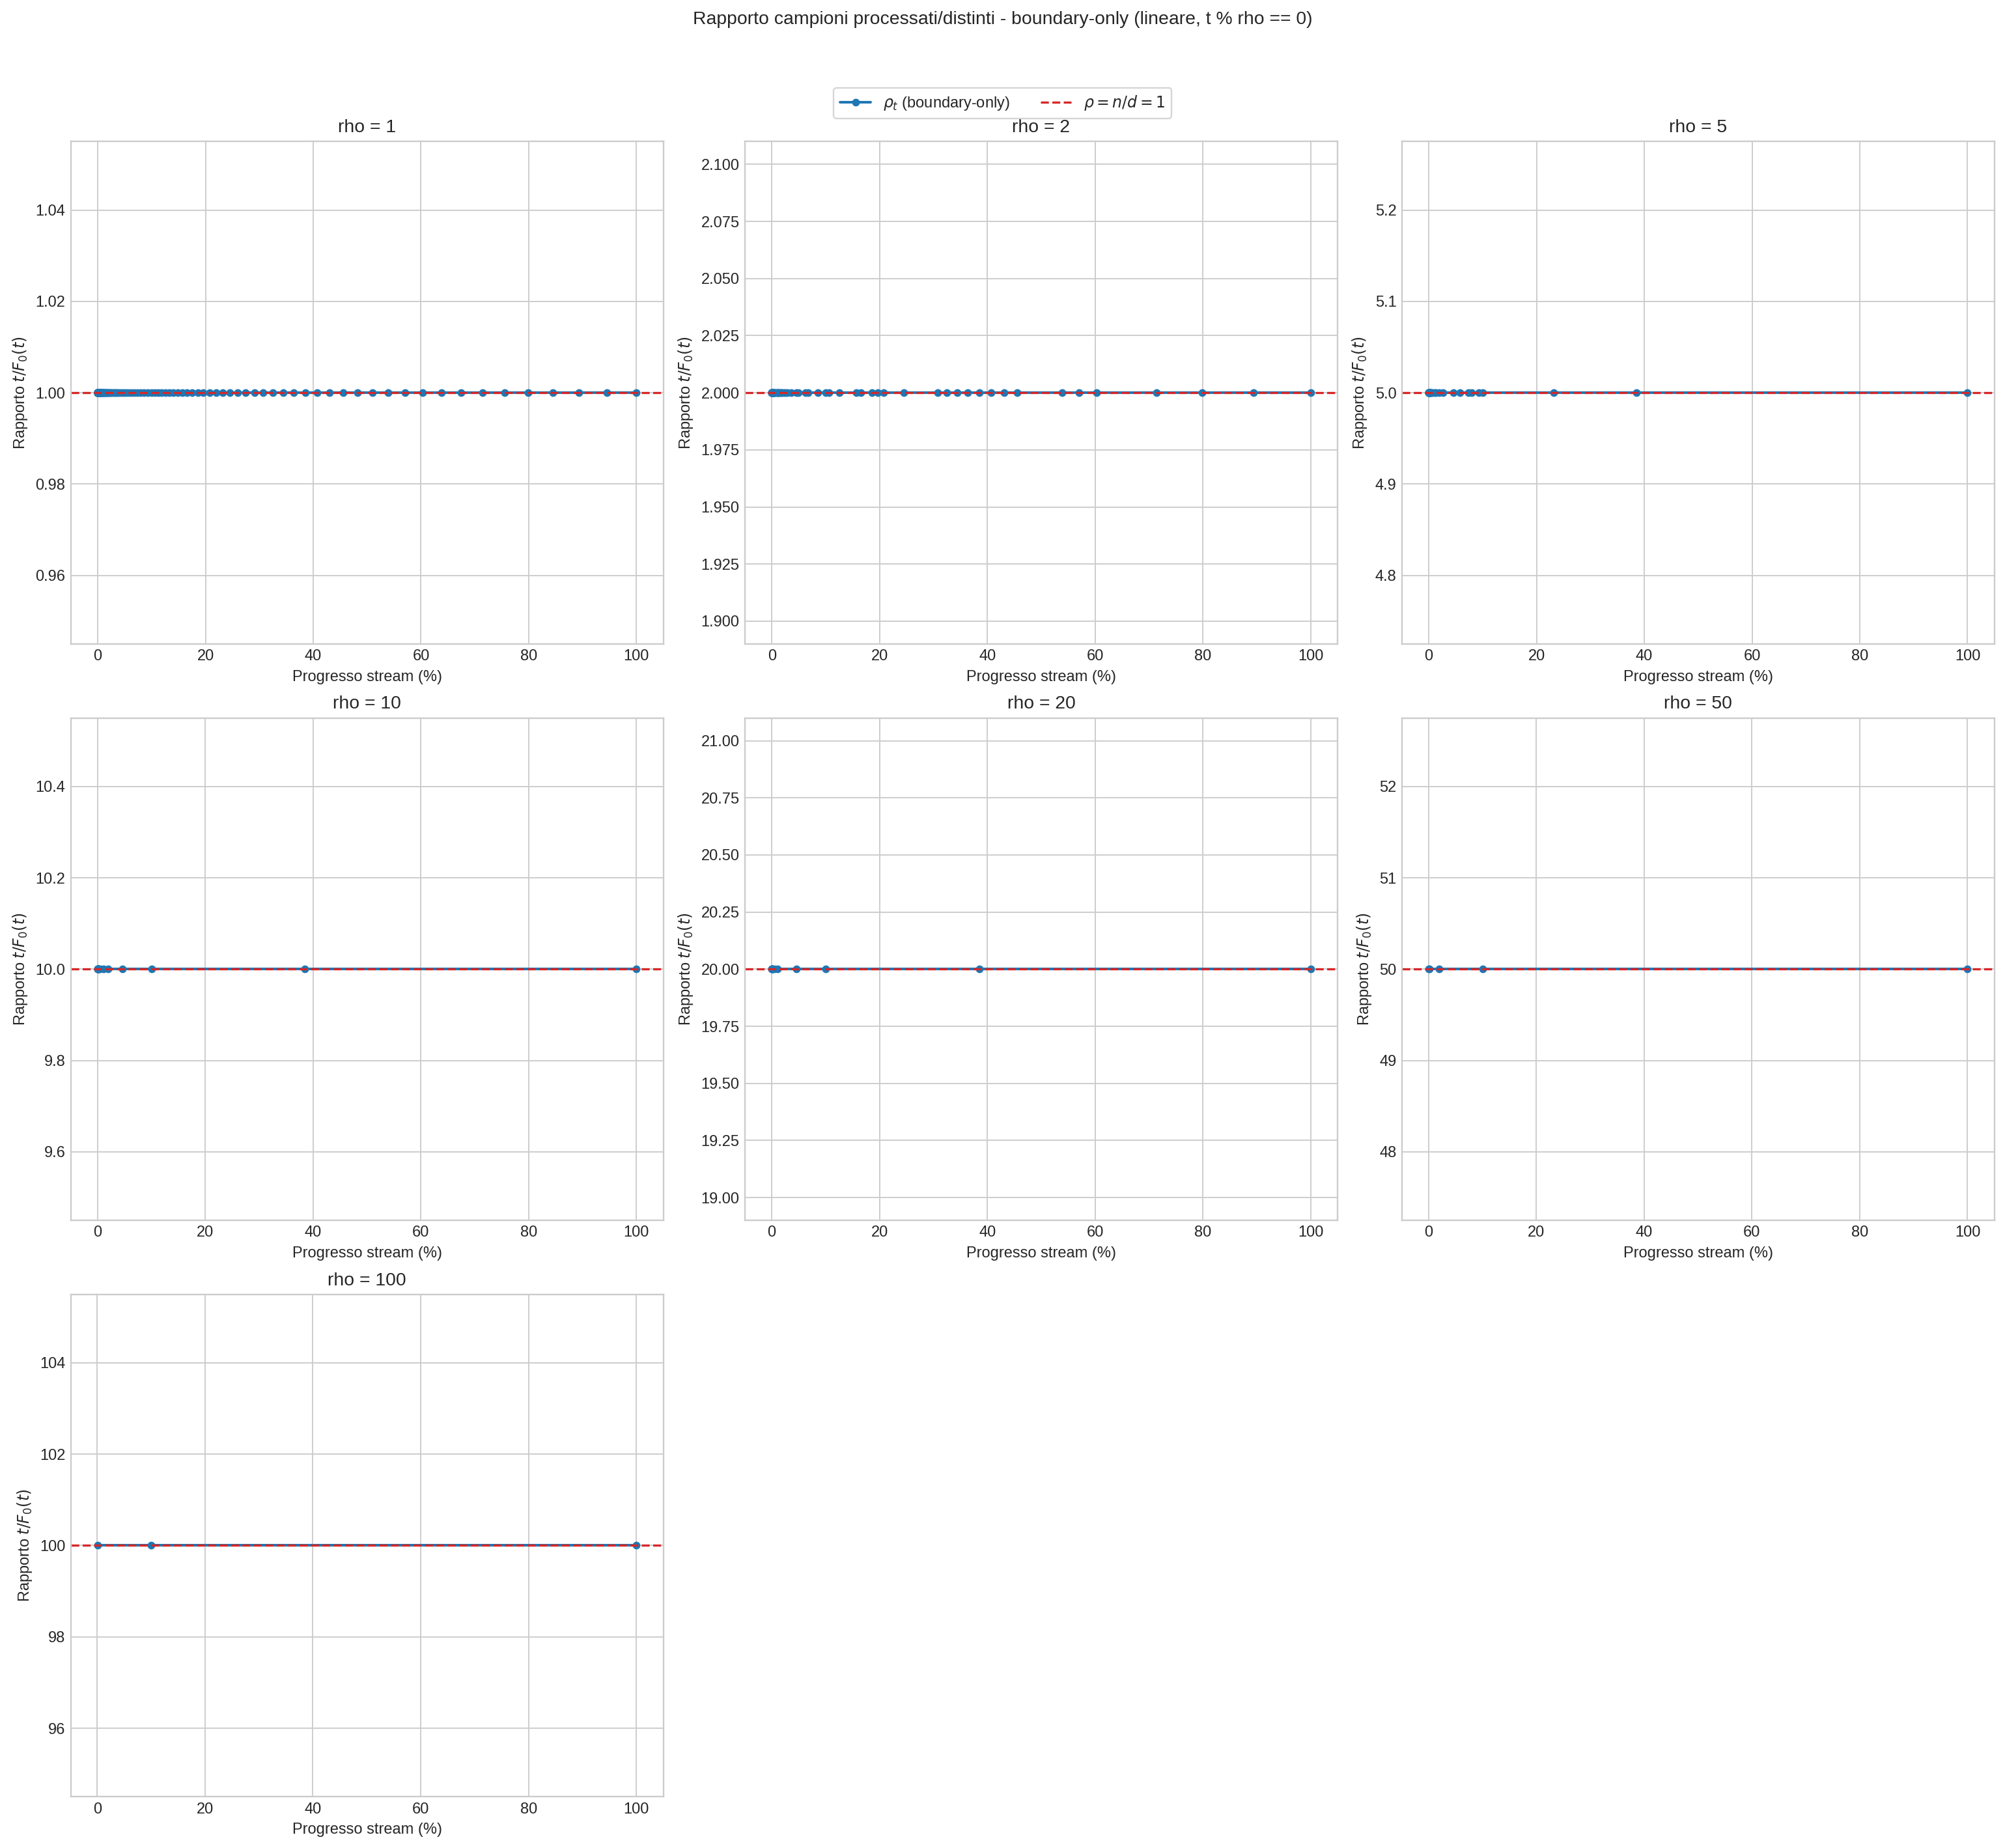
\includegraphics[width=\linewidth]{ratio_processed_vs_distinct_streaming_boundary_linear.png}

      \vspace{0.1cm}
      \scriptsize
      La validazione empirica conferma il comportamento atteso di \(\rho_t=t/\Fzero(t)\) ai bordi di blocco.
  \end{columns}

  \vspace{0.1cm}
  \tiny
  Test dedicati coprono algoritmi, merge, framework, schema CSV e generatore del dataset.
\end{frame}

\begin{frame}{Disegno sperimentale}
  \small
  \begin{itemize}
    \item Ambiente di test: AMD Ryzen 7 9700X, 32 GB DDR5, Clang 22.1.1, CMake 4.3.0.
    \item Tre modalit\`a di valutazione:
    \begin{itemize}
      \item \textbf{streaming}: andamento della stima lungo i prefissi;
      \item \textbf{merge omogeneo}: confronto tra merge e riferimento seriale;
      \item \textbf{merge eterogeneo}: casi \texttt{valid}, \texttt{recoverable}, \texttt{invalid}.
    \end{itemize}
    \item Due viste complementari in streaming:
    \begin{itemize}
      \item caso A: stima in funzione della cardinalit\`a reale del prefisso;
      \item caso B: stima in funzione di \(\rho_t = t/\Fzero(t)\) a cardinalit\`a target fissata.
    \end{itemize}
    \item Metriche principali: stima media, dispersione della stima, errore relativo medio ai punti finali.
    \item Gli esperimenti di merge sono concentrati su HyperLogLog++.
  \end{itemize}
\end{frame}

\begin{frame}{Risultato 1: comportamento degli algoritmi in streaming}
  \begin{columns}[T,totalwidth=\textwidth]
    \column{0.60\textwidth}
      \centering
      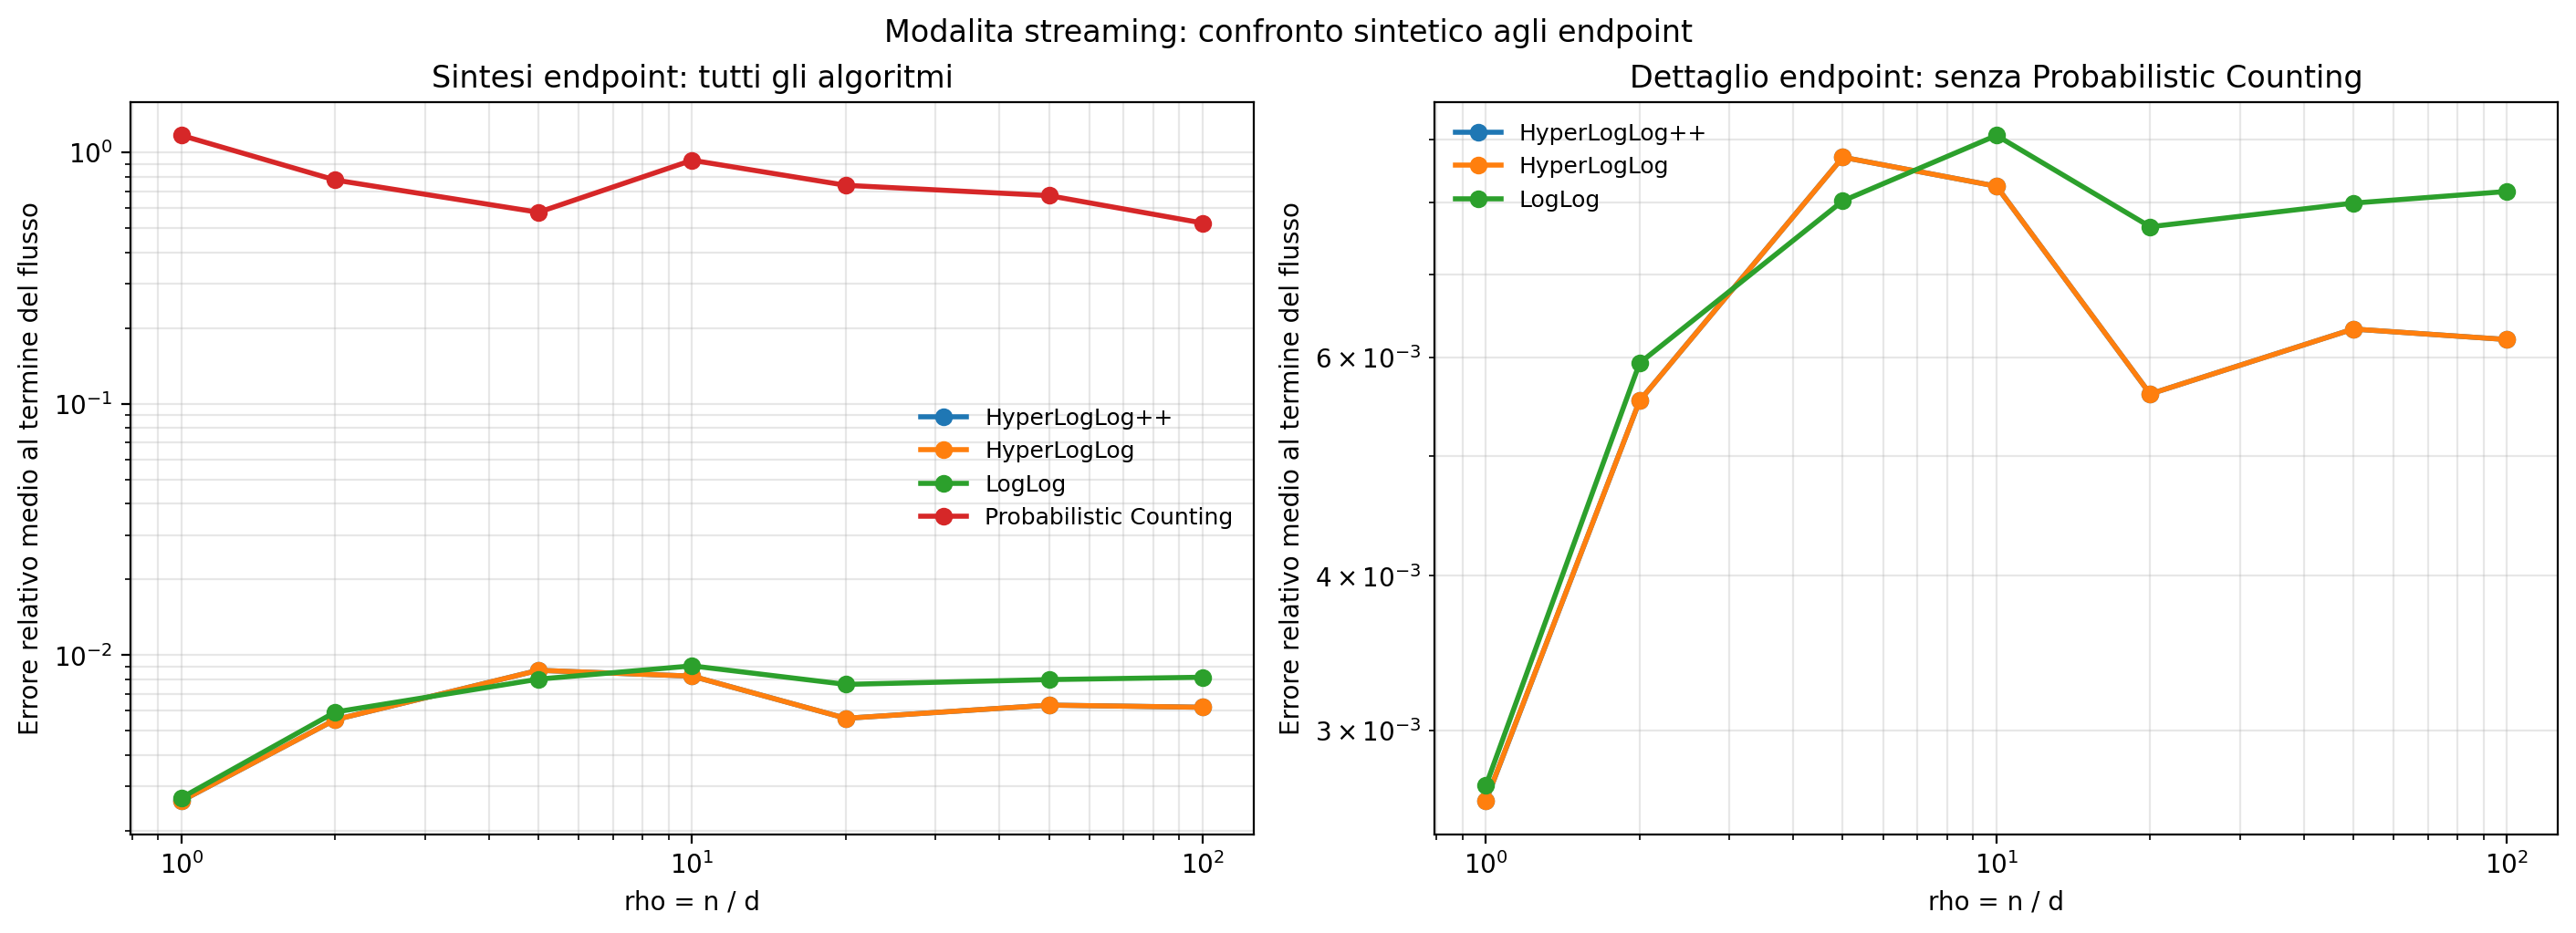
\includegraphics[width=\linewidth]{streaming_endpoint_mre_summary.png}
    \column{0.40\textwidth}
      \small
      \begin{itemize}
        \item Nella vista su \(\Fzero(t)\), HLL e HLL++ risultano quasi sovrapposti, con errore medio finale di circa \(0.00618\).
        \item Nella vista su \(\rho_t\), HLL++ \`e il migliore con circa \(3.95 \cdot 10^{-4}\), seguito da HLL con \(2.08 \cdot 10^{-3}\).
        \item LogLog \`e pi\`u sensibile e nella seconda vista raggiunge circa \(1.455\).
        \item Probabilistic Counting resta molto instabile nel dominio osservato, con circa \(0.770\) nella prima vista e \(0.346\) nella seconda.
      \end{itemize}
  \end{columns}
\end{frame}

\begin{frame}{Risultato 2: l'aumento di precisione favorisce soprattutto HLL++}
  \begin{columns}[T,totalwidth=\textwidth]
    \column{0.60\textwidth}
      \centering
      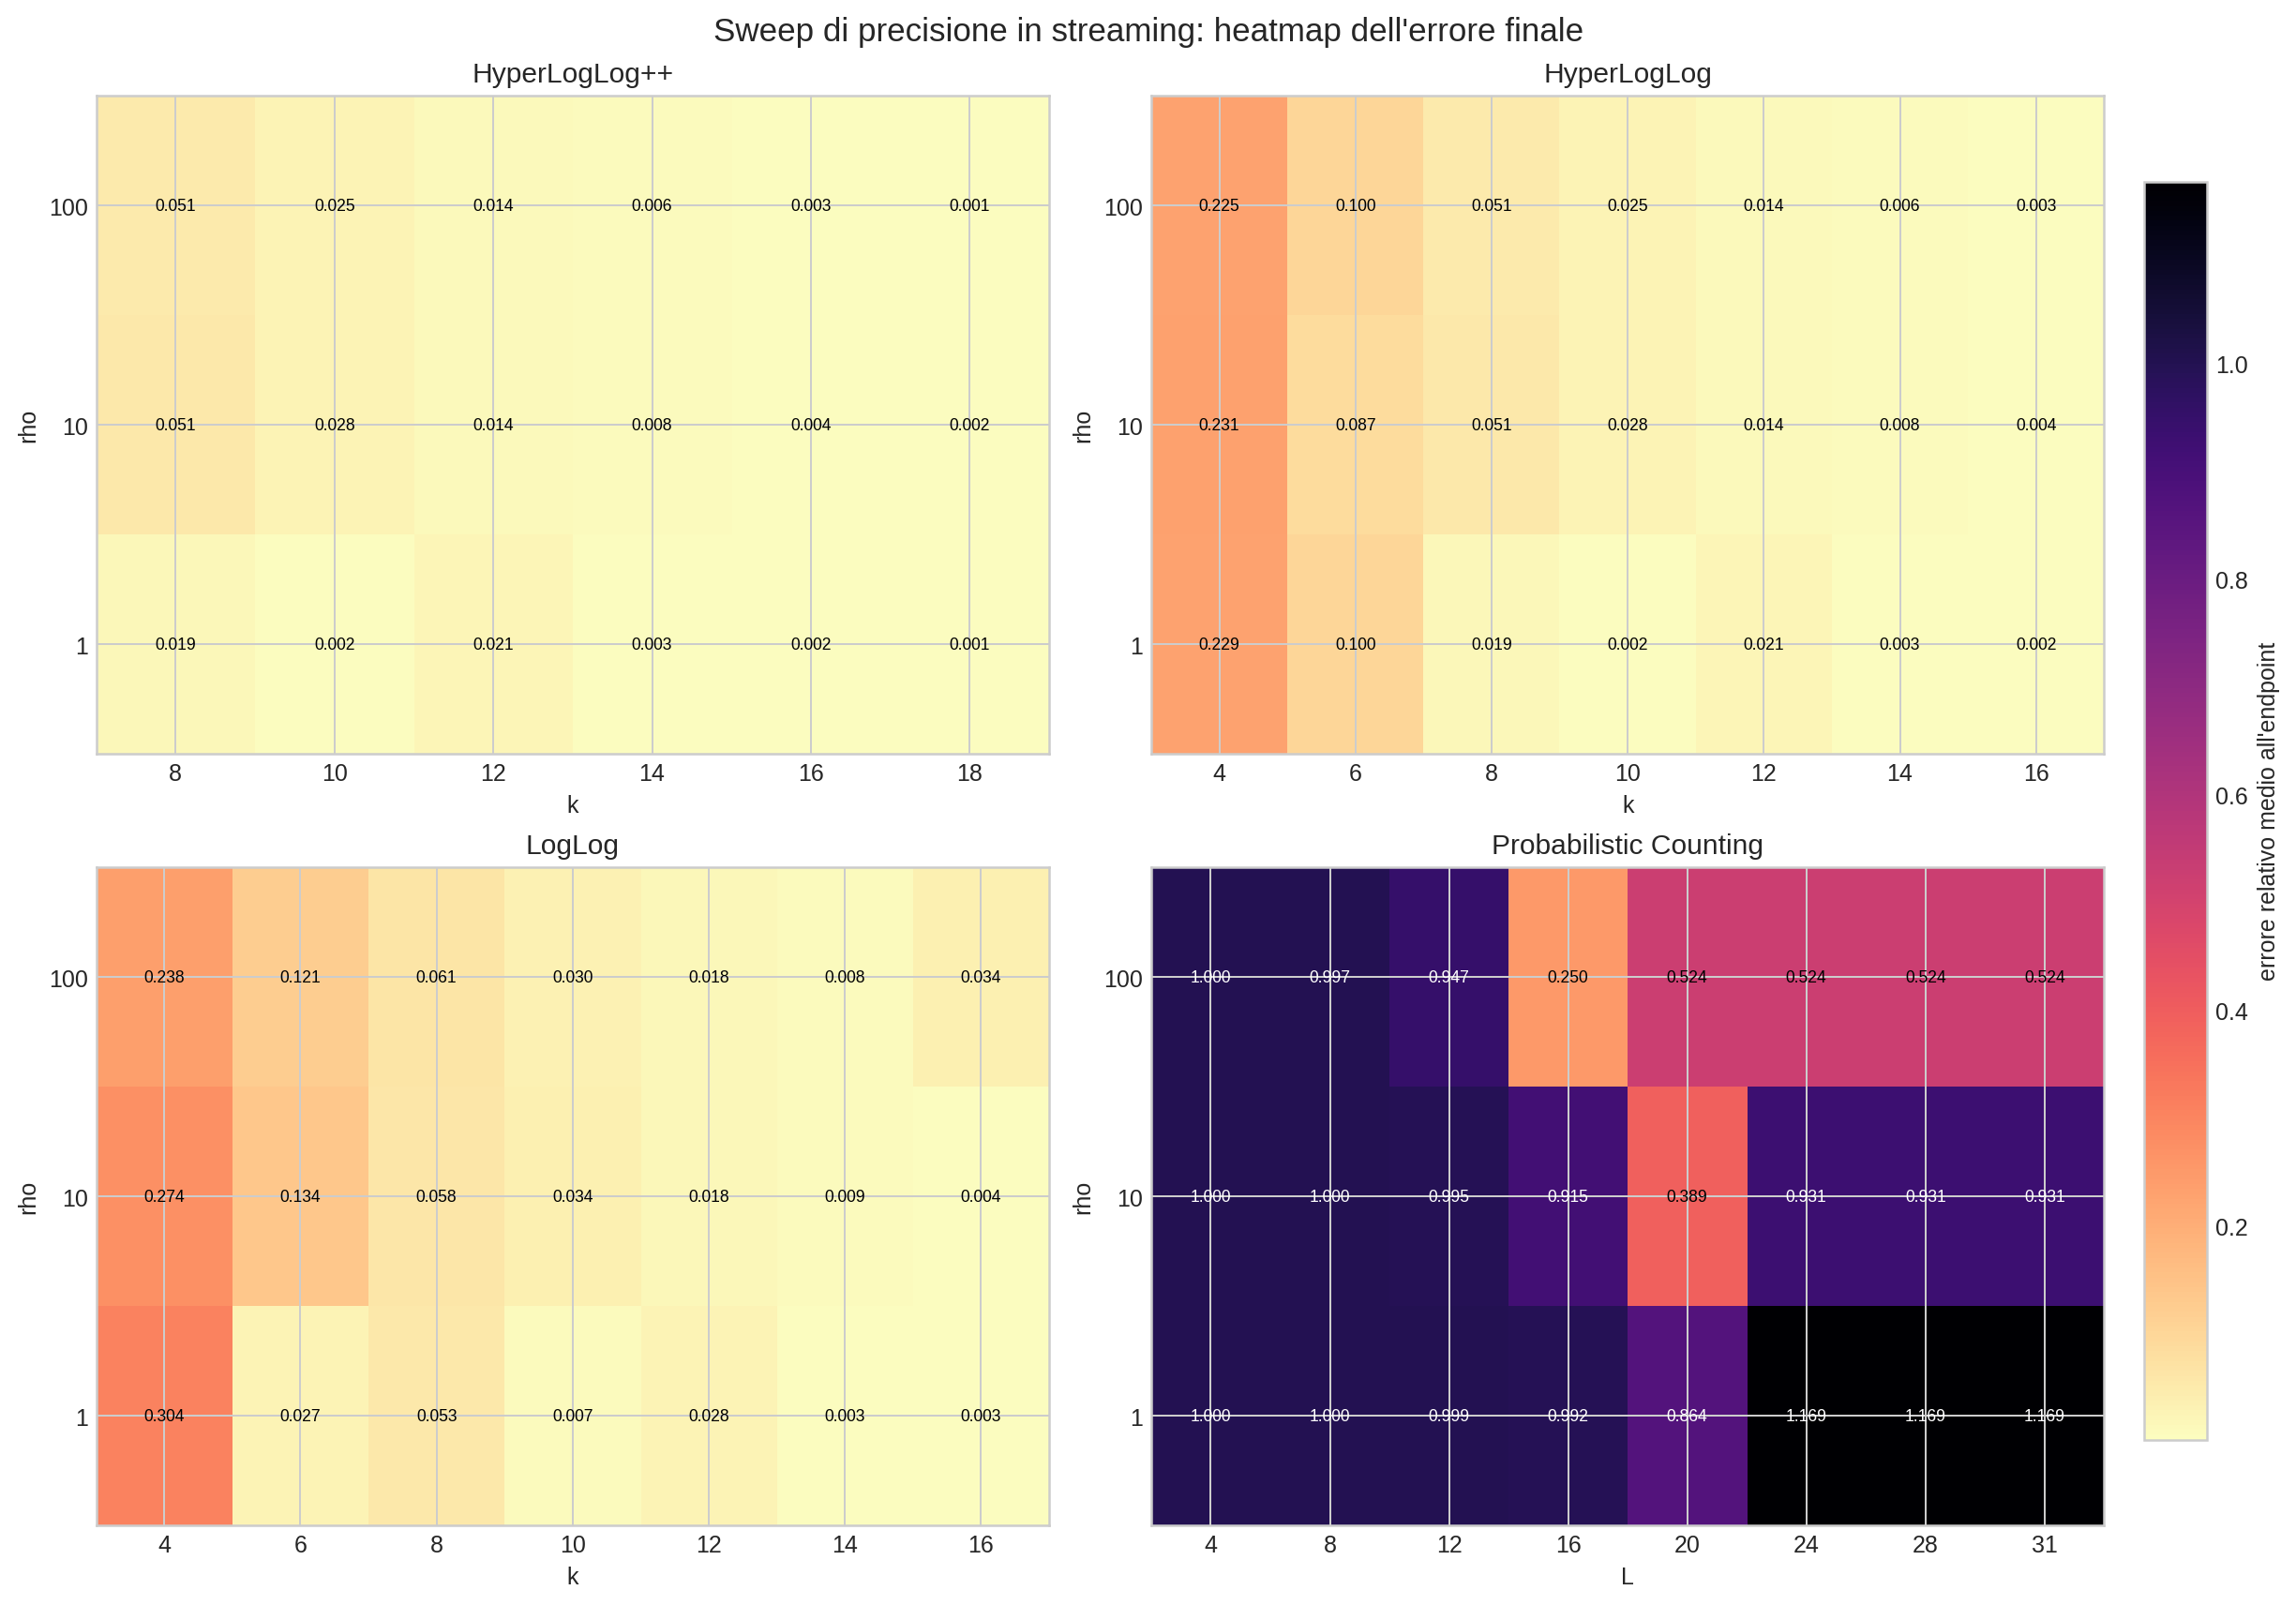
\includegraphics[width=\linewidth]{streaming_precision_sweep_endpoint_heatmaps.png}
    \column{0.40\textwidth}
      \tiny
      \begin{tabular}{p{0.9cm} p{0.8cm} p{2.0cm}}
        \toprule
        Algoritmo & Migliore & Osservazione \\
        \midrule
        HLL++ & \(k=18\) & migliore per tutti i valori di \(\rho\) osservati \\
        HLL & \(k=16\) & in media \(k=16\), ma con \(\rho=1\) basta \(k=10\) \\
        LogLog & \(k=14\) & andamento pi\`u irregolare; con \(\rho=10\) emerge \(k=16\) \\
        PC & \(L=20\) & migliora poco; con \(\rho=100\) emerge \(L=16\) \\
        \bottomrule
      \end{tabular}

      \vspace{0.2cm}
      \scriptsize
      \begin{itemize}
        \item HLL++ \`e il metodo con andamento pi\`u regolare e prevedibile.
        \item HLL migliora, ma meno uniformemente.
        \item LogLog e Probabilistic Counting mostrano dipendenza pi\`u marcata dal parametro.
      \end{itemize}
  \end{columns}
\end{frame}

\begin{frame}{Risultato 3: il merge omogeneo \`e il controllo del caso \texttt{valid}}
  \begin{itemize}
    \item Configurazione: HyperLogLog++, \(\rho \in \{1,10,100\}\), \(k \in \{10,14,18\}\), quattro funzioni di hash.
    \item Condizione di omogeneit\`a: stessa funzione di hash, stesso seed e stessi parametri sui due lati.
    \item Totale osservato: 36 configurazioni e 900 coppie di merge.
  \end{itemize}

  \vspace{0.15cm}
  \[
    \Delta_{abs}=0, \qquad \Delta_{rel}=0
  \]

  \small
  \begin{tabular}{ccccc}
    \toprule
    \(\rho\) & \(d\) & Coppie totali & Coppie con delta \(\neq 0\) & Max \(\Delta_{rel}\) \\
    \midrule
    1 & \(10^7\) & 300 & 0 & 0 \\
    10 & \(10^6\) & 300 & 0 & 0 \\
    100 & \(10^5\) & 300 & 0 & 0 \\
    \bottomrule
  \end{tabular}
\end{frame}

\begin{frame}{Risultato 4: hash mismatch = caso \texttt{invalid}}
  \begin{columns}[T,totalwidth=\textwidth]
    \column{0.60\textwidth}
      \centering
      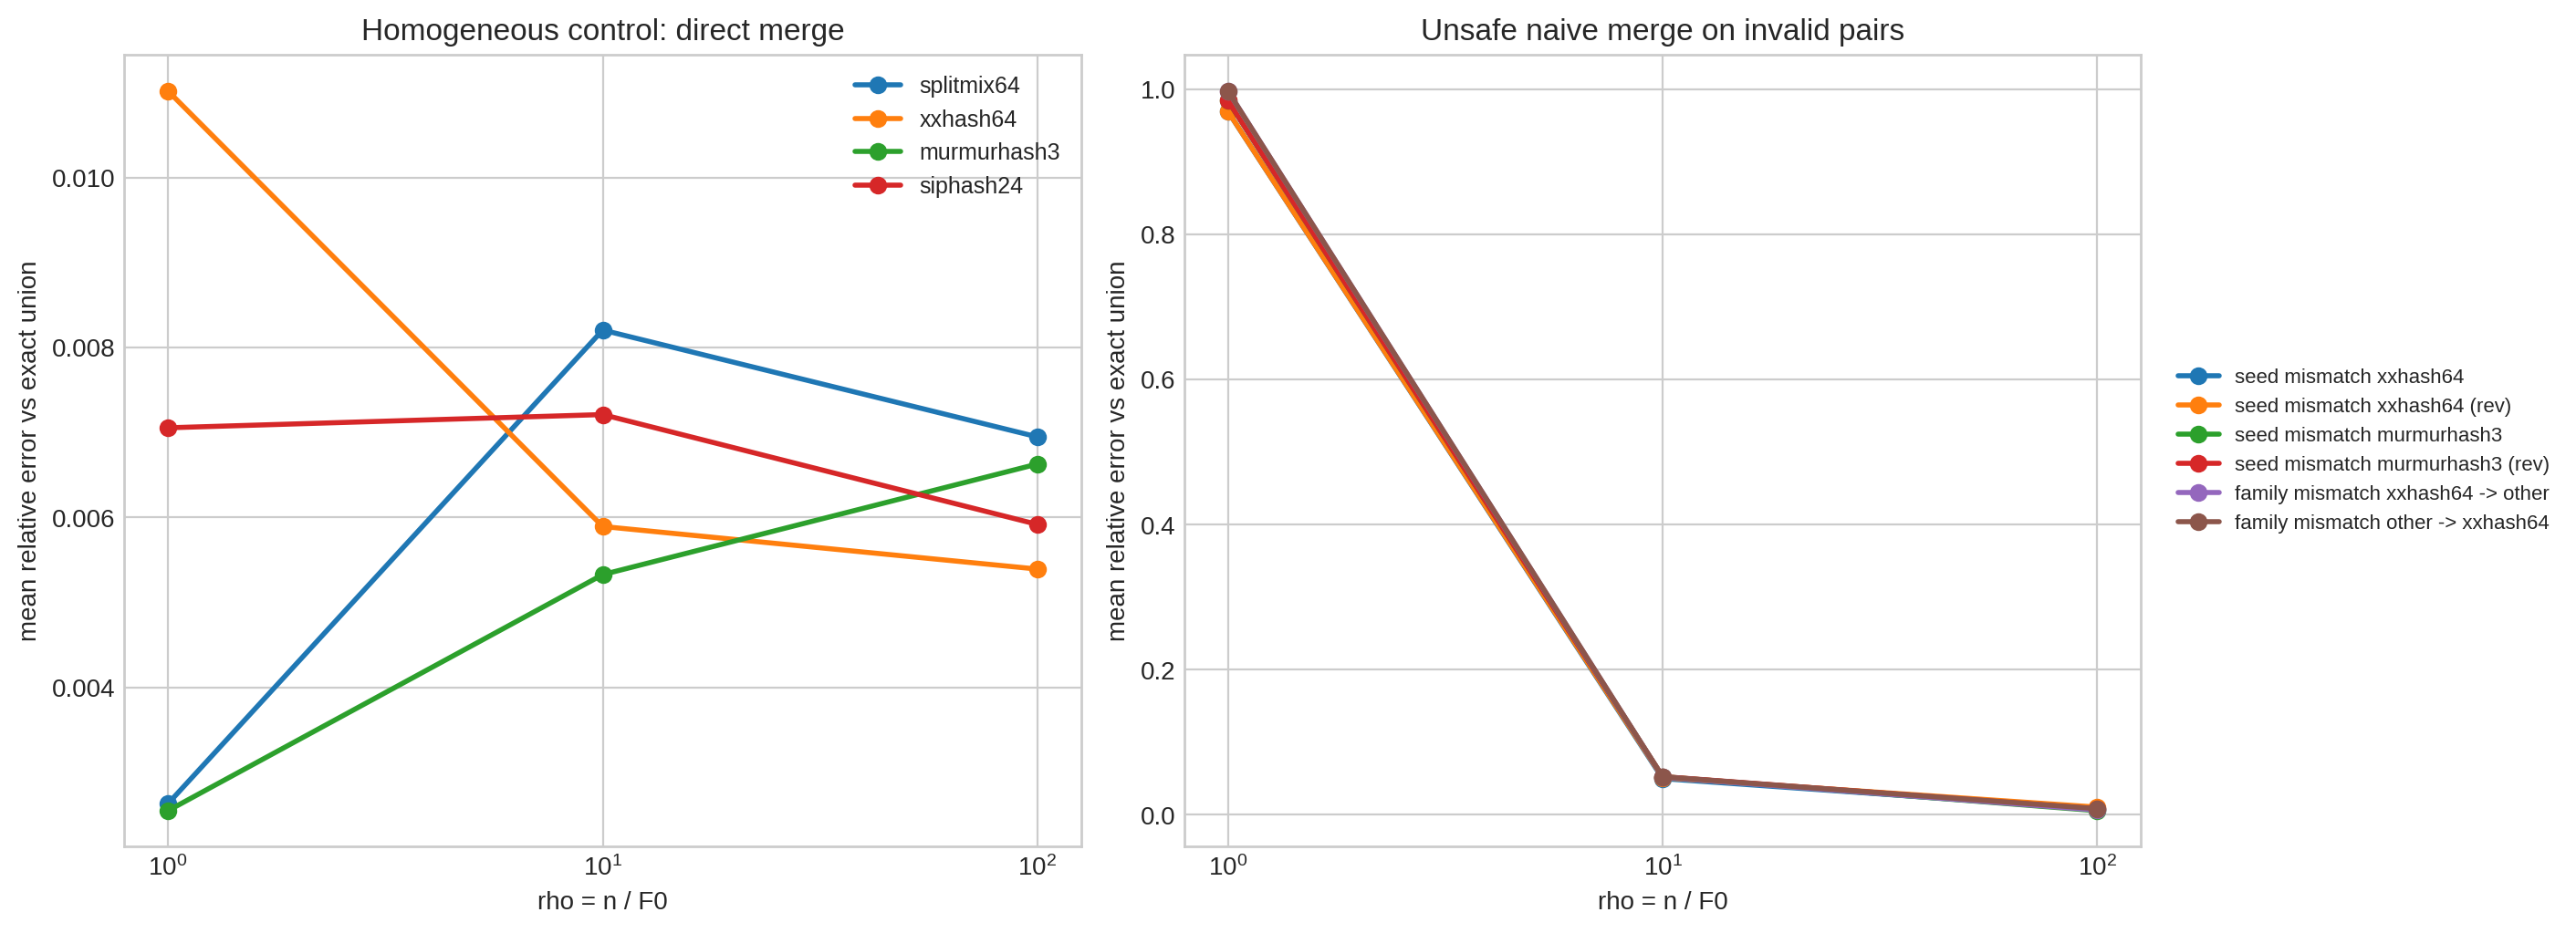
\includegraphics[width=\linewidth]{merge_hpp_hash_mismatch_overview.png}
    \column{0.40\textwidth}
      \scriptsize
      \begin{itemize}
        \item Scenari osservati: seed mismatch su \texttt{xxhash64}/\texttt{murmurhash3} e family mismatch tra le quattro hash supportate.
        \item Controllo omogeneo locale: errore medio \(=0.006233\).
        \item Casi \texttt{invalid}: errore medio tra \(0.342374\) e \(0.352802\).
        \item Errore massimo osservato: \(1.009634\).
      \end{itemize}

      \begin{alertblock}{Conclusione}
        Se cambia la semantica dell'hash, il merge forzato perde significato. In questo contesto il caso va rifiutato.
      \end{alertblock}
  \end{columns}
\end{frame}

\begin{frame}{Risultato 5: precision mismatch = caso \texttt{recoverable}}
  \begin{columns}[T,totalwidth=\textwidth]
    \column{0.59\textwidth}
      \centering
      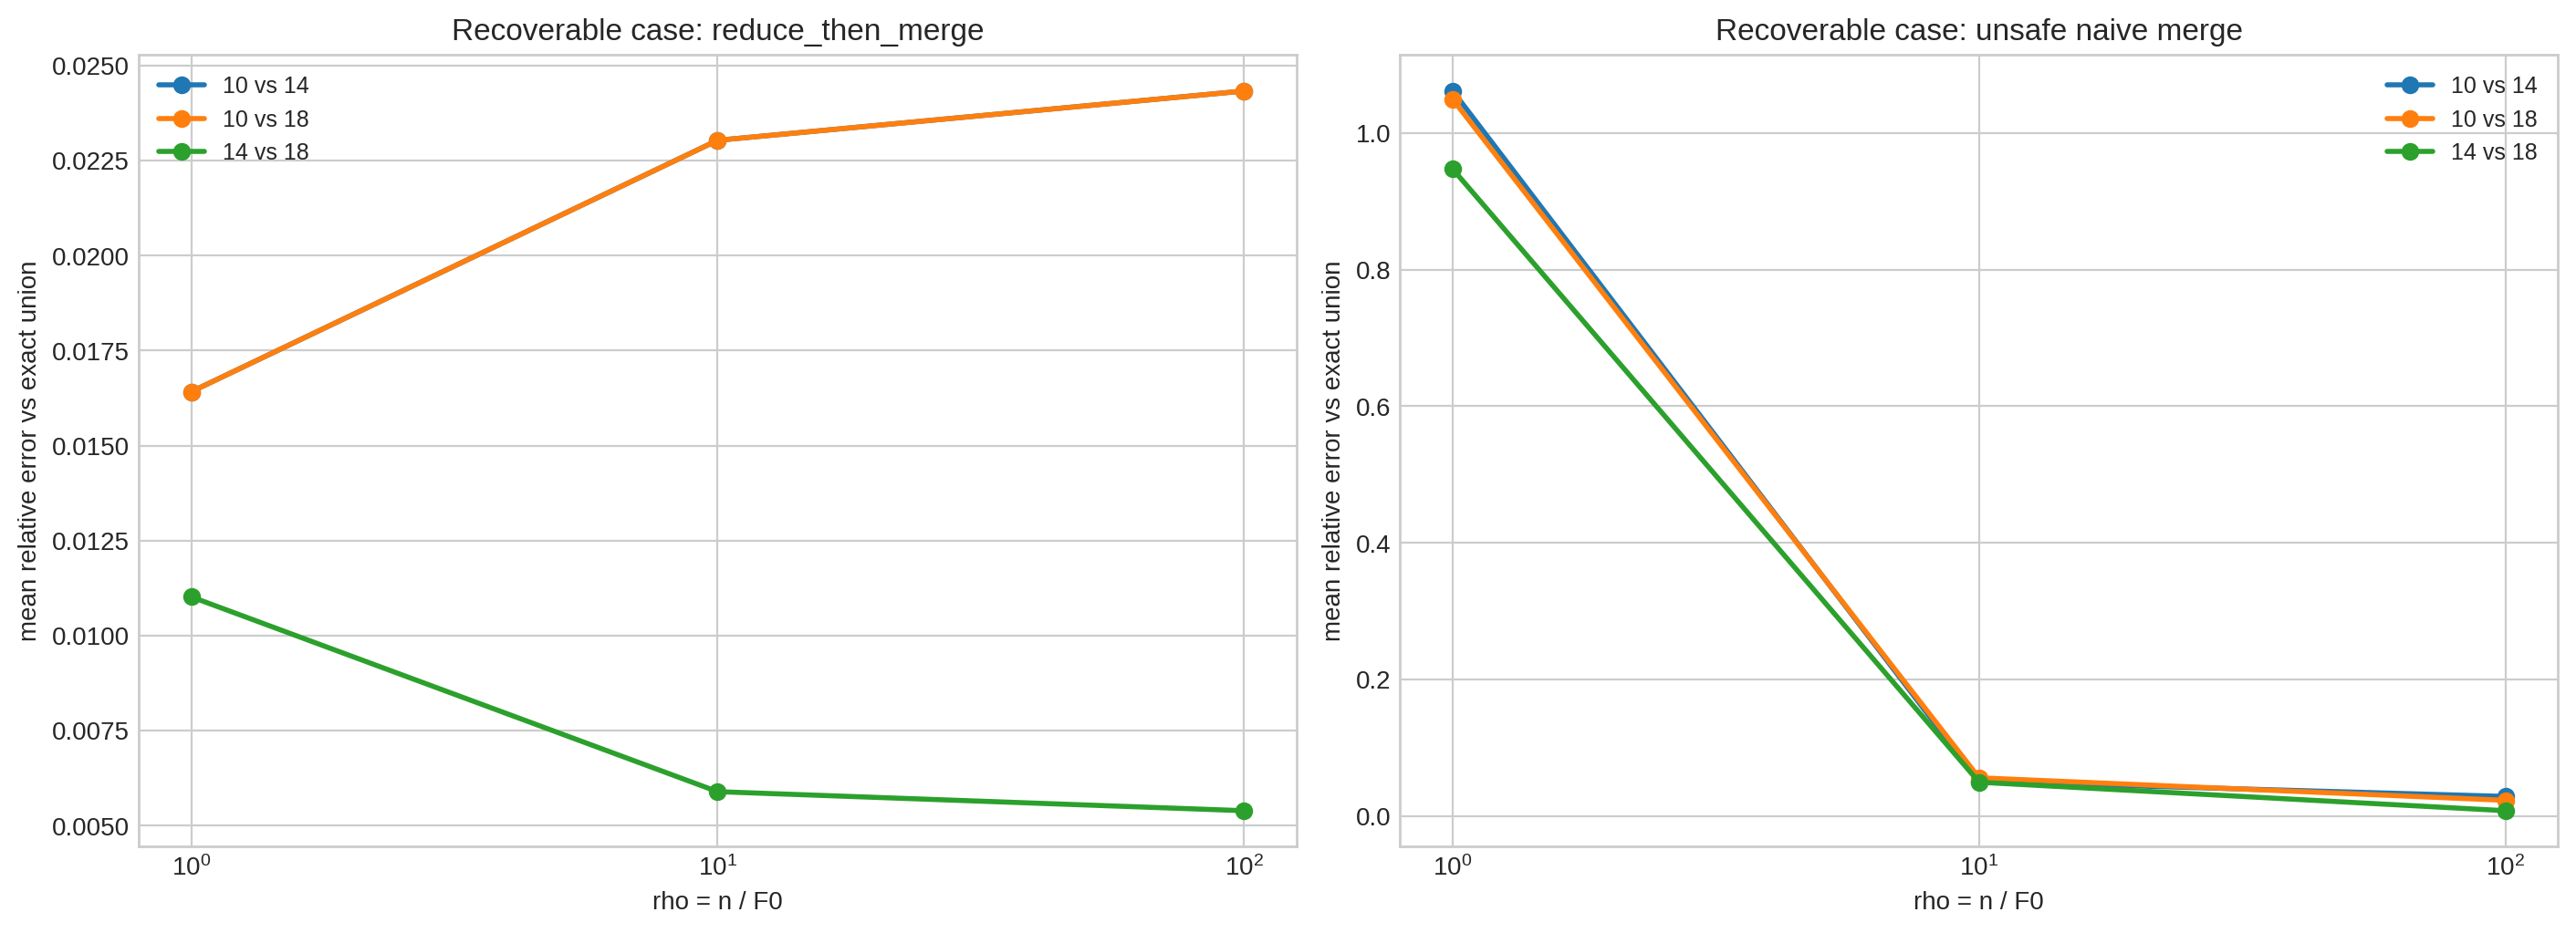
\includegraphics[width=\linewidth]{merge_hpp_precision_mismatch_overview.png}
    \column{0.41\textwidth}
      \small
      \begin{itemize}
        \item Hash fissata a \texttt{xxhash64}, stesso seed, coppie \((10,14)\), \((10,18)\), \((14,18)\) e versioni invertite.
        \item \texttt{reject}: nessuna stima di merge, riferimento seriale \(=0.016651\).
      \end{itemize}

      \scriptsize
      \begin{tabular}{p{2.1cm} p{1.8cm}}
        \toprule
        Strategia & \(\overline{\varepsilon}_{merge}\) \\
        \midrule
        \begin{tabular}[t]{@{}l@{}}\texttt{unsafe\_naive\_}\\\texttt{merge}\end{tabular} & \(0.363882\) \\
        \begin{tabular}[t]{@{}l@{}}\texttt{reduce\_then\_}\\\texttt{merge}\end{tabular} & \(0.016651\) \\
        \bottomrule
      \end{tabular}

      \vspace{0.15cm}
      \small
      \begin{itemize}
        \item \texttt{reduce\_then\_merge} coincide con il riferimento seriale e con il baseline omogeneo a precisione minima.
        \item Il merge forzato raggiunge massimo \(1.061378\) e degrado medio \(32.37\).
      \end{itemize}
  \end{columns}
\end{frame}

\begin{frame}{Sintesi dei risultati e contributi}
  \begin{columns}[T,totalwidth=\textwidth]
    \column{0.50\textwidth}
      \begin{block}{Risultati empirici}
        \begin{itemize}
          \item HLL++ \`e il metodo pi\`u stabile nel dominio osservato.
          \item Il merge omogeneo coincide col riferimento seriale.
          \item L'eterogeneit\`a dell'hash rompe la correttezza del merge.
          \item Il mismatch di precisione \`e recuperabile solo tramite normalizzazione esplicita.
        \end{itemize}
      \end{block}
    \column{0.50\textwidth}
      \begin{block}{Contributi del lavoro}
        \begin{itemize}
          \item Implementazione uniforme di pi\`u algoritmi count-distinct.
          \item Interfaccia comune per hash, dataset, metriche e serializzazione.
          \item Framework riutilizzabile per streaming e merge distribuito.
          \item Lessico operativo \texttt{valid}/\texttt{recoverable}/\texttt{invalid}.
        \end{itemize}
      \end{block}
  \end{columns}

  \begin{alertblock}{Take-away}
    Negli sketch count-distinct distribuiti, hash e parametri fanno parte della semantica dello sketch: senza compatibilit\`a semantica il merge non \`e un'operazione neutra.
  \end{alertblock}
\end{frame}

\begin{frame}{Limiti e sviluppi futuri}
  \begin{columns}[T,totalwidth=\textwidth]
    \column{0.48\textwidth}
      \begin{block}{Limiti del lavoro}
        \begin{itemize}
          \item Dataset soprattutto sintetico e controllato
          \item Studio del merge concentrato soprattutto su casi pairwise
          \item Analisi eterogenea limitata a hash mismatch e precision mismatch
          \item Parte di merge sviluppata soprattutto su HLL++
        \end{itemize}
      \end{block}
    \column{0.48\textwidth}
      \begin{block}{Direzioni future}
        \begin{itemize}
          \item Dati reali e integrazione con sorgenti come Apache Kafka
          \item Topologie distribuite pi\`u ampie e scelta del punto ottimale di riduzione alla precisione minima
          \item Altri assi di eterogeneit\`a semanticamente chiari
          \item Algoritmi pi\`u recenti come UltraLogLog, SetSketch, HyperLogLogLog
          \item Estensione del framework a Bloom filter, Count-Min Sketch e ad altri costi di merge
        \end{itemize}
      \end{block}
  \end{columns}
\end{frame}

\begin{frame}{Domande}
  \centering
  \Large Grazie per l'attenzione.
\end{frame}

\end{document}
